\documentclass[17pt,a4paper,landscape]{extarticle}
\usepackage[margin=2.35cm,top=0.12cm,left=1.05cm]{geometry}
\usepackage{amsmath}
\usepackage{amssymb}
\usepackage{tasks}
\usepackage{tikz}
\usepackage{xcolor}
\usepackage[sfdefault,lf]{FiraSans}
\renewcommand{\familydefault}{\sfdefault}
\setlength{\parindent}{0pt}
\pagestyle{empty}
\settasks{label=\textbf{\arabic*.}, label-width=2.2em, item-indent=2.95em, column-sep=2.1cm, after-item-skip=4.7em}
\renewcommand{\arraystretch}{1.15}
\everymath{\displaystyle}

\begin{document}
\sffamily
\boldmath

\boldmath

\boldmath

\boldmath

{\LARGE \textbf{Angles on a straight line --- Excellence}}
\begin{tasks}(3)
\task {Find \mbox{$x$}.\\[0.4em]
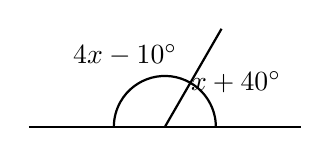
\begin{tikzpicture}[scale=0.72,baseline=(current bounding box.center)]
\draw[thick] (-2.4,0)--(0,0)--(2.4,0);
\draw[thick] (0,0)--({2*cos(60)},{2*sin(60)});
\draw[thick] (0.9,0) arc[start angle=0,end angle=60,radius=0.9];
\draw[thick] ({0.9*cos(60)},{0.9*sin(60)}) arc[start angle=60,end angle=180,radius=0.9];
\node at ({1.45*cos(30)},{1.45*sin(30)+0.06}) {$x+40^\circ$};
\node at ({1.4*cos(120)},{1.4*sin(120)+0.06}) {$4x-10^\circ$};
\end{tikzpicture}}
\task {Find \mbox{$y$}.\\[0.4em]
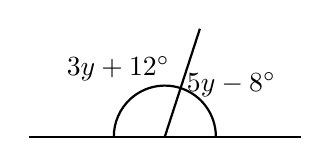
\begin{tikzpicture}[scale=0.72,baseline=(current bounding box.center)]
\draw[thick] (-2.4,0)--(0,0)--(2.4,0);
\draw[thick] (0,0)--({2*cos(72)},{2*sin(72)});
\draw[thick] (0.9,0) arc[start angle=0,end angle=72,radius=0.9];
\draw[thick] ({0.9*cos(72)},{0.9*sin(72)}) arc[start angle=72,end angle=180,radius=0.9];
\node at ({1.45*cos(36)},{1.45*sin(36)+0.06}) {$5y-8^\circ$};
\node at ({1.4*cos(126)},{1.4*sin(126)+0.06}) {$3y+12^\circ$};
\end{tikzpicture}}
\task {Find \mbox{$a$}.\\[0.4em]
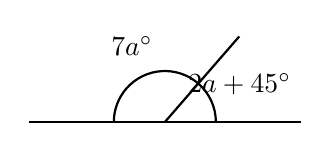
\begin{tikzpicture}[scale=0.72,baseline=(current bounding box.center)]
\draw[thick] (-2.4,0)--(0,0)--(2.4,0);
\draw[thick] (0,0)--({2*cos(49)},{2*sin(49)});
\draw[thick] (0.9,0) arc[start angle=0,end angle=49,radius=0.9];
\draw[thick] ({0.9*cos(49)},{0.9*sin(49)}) arc[start angle=49,end angle=180,radius=0.9];
\node at ({1.45*cos(24.5)},{1.45*sin(24.5)+0.06}) {$2a+45^\circ$};
\node at ({1.4*cos(114.5)},{1.4*sin(114.5)+0.06}) {$7a^\circ$};
\end{tikzpicture}}
\task {A student says \mbox{$118^\circ$} and \mbox{$72^\circ$} are angles on a straight line because both are obtuse. Explain why this is wrong.}
\task {Two adjacent angles on a straight line are in the ratio \mbox{$2:7$}. Find both angles.}
\task {Two adjacent angles on a straight line are in the ratio \mbox{$4:5$}. Find both angles.}
\task {One angle is \mbox{$14^\circ$} less than twice the other. Find both angles.}
\task {One angle is \mbox{$38^\circ$} more than half the other. Find both angles.}
\task {Three angles lie along a straight line. Two are \mbox{$35^\circ$} and \mbox{$68^\circ$}. Find the third angle.}
\task {Three angles lie along a straight line. They are \mbox{$x^\circ$}, \mbox{$2x^\circ$} and \mbox{$3x^\circ$}. Find \mbox{$x$}.}
\task {Three angles lie along a straight line. They are \mbox{$(x+10)^\circ$}, \mbox{$(x+20)^\circ$} and \mbox{$50^\circ$}. Find \mbox{$x$}.}
\task {A straight line is split into four adjacent angles: \mbox{$25^\circ$}, \mbox{$y^\circ$}, \mbox{$40^\circ$} and \mbox{$2y^\circ$}. Find \mbox{$y$}.}
\task {A straight line is split into four adjacent angles: \mbox{$a^\circ$}, \mbox{$(a+15)^\circ$}, \mbox{$2a^\circ$} and \mbox{$30^\circ$}. Find \mbox{$a$}.}
\task {Can two acute angles make a straight line? Explain your answer.}
\task {Can an obtuse angle and a reflex angle lie adjacent on one straight line? Explain your answer.}
\task {Write your own pair of adjacent angles on a straight line where one angle is algebraic and the other is numeric. Then solve it.}
\end{tasks}

\end{document}
